% questions.tex —— 2018 年上海市春季高考数学试卷 · 题目内容片段（无答案）
% 由 tools/generate_projects.py 依来源总账自 2018/2018_数学真题_春季上海_试题.md 生成，勿手改（改源 MD 后重跑）


\begin{gktip}
\textbf{来源与核对边界}：题面依据固定来源 PDF 第 1–6 页逐题转录，source ID 与 SHA-256 见 frontmatter。来源文件自题年份、上海市和春季高考，并标注日期 \texttt{2018.01}；出版者、版次、官方来源链尚未核实。固定 PDF 第 7 页另有“参考答案”，本题面稿不将其混入题目，也不据此称答案为官方。

\textbf{原文待核}：Q17 在“已知 $y=\cos x$”后直接使用 $f$；Q18 写“点 $(2,1)$ 在上”而未在该处指明所属曲线，均照录原文，不擅自补字。Q21(3)原卷印有“前 $n$ 项和”，已按源页更正转录。Q7、Q12、Q14、Q19的数学图已按原图关系矢量重绘；Q19现场照片保留固定源第4页的原始裁片，作为情境照片而不作矢量化。
\end{gktip}

\gkpart{一、填空题}

（本大题共 12 题，满分 54 分，第 1–6 题每题 4 分，第 7–12 题每题 5 分。）

\begin{question}
\gkti{1}不等式 $|x|>1$ 的解集为 $\underline{\qquad}$。

\end{question}
\begin{question}
\gkti{2}计算：$\displaystyle\lim_{n\to\infty}\frac{3n-1}{n+2}=\underline{\qquad}$。

\end{question}
\begin{question}
\gkti{3}设集合 $A=\{x\mid 0<x<2\}$，$B=\{x\mid -1<x<1\}$，则 $A\cap B=\underline{\qquad}$。

\end{question}
\begin{question}
\gkti{4}若复数 $z=1+i$（$i$ 是虚数单位），则 $z+\dfrac{2}{z}=\underline{\qquad}$。

\end{question}
\begin{question}
\gkti{5}已知 $\{a_n\}$ 是等差数列，若 $a_2+a_8=10$，则 $a_3+a_5+a_7=\underline{\qquad}$。

\end{question}
\begin{question}
\gkti{6}已知平面上动点 $P$ 到两个定点 $(1,0)$ 和 $(-1,0)$ 的距离之和等于 $4$，则动点 $P$ 的轨迹方程为 $\underline{\qquad}$。

\Needspace{0.4\textheight}
\end{question}
\begin{question}
\gkti{7}如图，在长方体 $ABCD-A_1B_1C_1D_1$ 中，$AB=3$，$BC=4$，$AA_1=5$，$O$ 是 $A_1C_1$ 的中点，则三棱锥 $A-A_1OB_1$ 的体积为 $\underline{\qquad}$。
\nopagebreak[4]
\begin{center}% Source: src-b19b233abb266d1b051ded3c332a399c1722d8192d07ce1bf2234dda57bd25bc, PDF p.1.
% Topology follows the source; oblique projection is schematic, not metric.
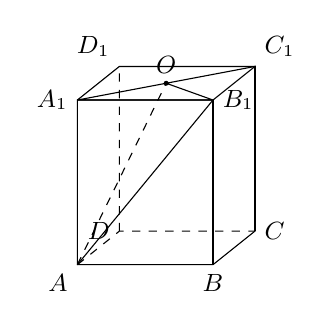
\begin{tikzpicture}[scale=0.82, every node/.style={font=\small}]
  \coordinate (A) at (0,0);
  \coordinate (B) at (2.1,0);
  \coordinate (C) at (2.75,0.52);
  \coordinate (D) at (0.65,0.52);
  \coordinate (A1) at (0,2.55);
  \coordinate (B1) at (2.1,2.55);
  \coordinate (C1) at (2.75,3.07);
  \coordinate (D1) at (0.65,3.07);
  \coordinate (O) at (1.375,2.81);
  \draw (A)--(B)--(C)--(C1)--(B1)--(A1)--cycle;
  \draw (C1)--(D1)--(A1);
  \draw[dashed] (A)--(D)--(C) (D)--(D1);
  \draw (A)--(A1) (B)--(B1) (C)--(C1);
  \draw (A1)--(C1) (A1)--(B1) (O)--(B1) (A)--(B1);
  \draw[dashed] (A)--(O);
  \fill (O) circle (1.1pt);
  \node[below left] at (A) {$A$};
  \node[below] at (B) {$B$};
  \node[right] at (C) {$C$};
  \node[left] at (D) {$D$};
  \node[left] at (A1) {$A_1$};
  \node[right] at (B1) {$B_1$};
  \node[above right] at (C1) {$C_1$};
  \node[above left] at (D1) {$D_1$};
  \node[above] at (O) {$O$};
\end{tikzpicture}
\end{center}
\nopagebreak[4]
\end{question}
\begin{question}
\gkti{8}某校组队参加辩论赛，从 6 名学生中选出 4 人分别担任一、二、三、四辩，若其中学生甲必须参赛且不担任四辩，则不同的安排方法种数为 $\underline{\qquad}$（结果用数值表示）。

\end{question}
\begin{question}
\gkti{9}设 $a\in\mathbb R$，若 $\left(x^2+\dfrac{2}{x}\right)^9$ 与 $\left(x+\dfrac{a}{x^2}\right)^9$ 的二项展开式中的常数项相等，则 $a=\underline{\qquad}$。

\end{question}
\begin{question}
\gkti{10}设 $m\in\mathbb R$，若 $z$ 是关于 $x$ 的方程 $x^2+mx+m^2-1=0$ 的一个虚根，则 $|z|$ 的取值范围是 $\underline{\qquad}$。

\end{question}
\begin{question}
\gkti{11}设 $a>0$，函数 $f(x)=x+2(1-x)\sin(ax)$，$x\in(0,1)$，若函数 $y=2x-1$ 与 $y=f(x)$ 的图像有且仅有两个不同的公共点，则 $a$ 的取值范围是 $\underline{\qquad}$。

\Needspace{0.4\textheight}
\end{question}
\begin{question}
\gkti{12}如图，正方形 $ABCD$ 的边长为 20 米，圆 $O$ 的半径为 1 米，圆心是正方形的中心，点 $P\text{、}Q$ 分别在线段 $AD\text{、}CB$ 上，若线段 $PQ$ 与圆 $O$ 有公共点，则称点 $Q$ 在点 $P$ 的“盲区”中，已知点 $P$ 以 1.5 米/秒的速度从 $A$ 出发向 $D$ 移动，同时，点 $Q$ 以 1 米/秒的速度从 $C$ 出发向 $B$ 移动，则在点 $P$ 从 $A$ 移动到 $D$ 的过程中，点 $Q$ 在点 $P$ 的盲区中的时长约为 $\underline{\qquad}$ 秒（精确到 0.1）。
\nopagebreak[4]
\begin{center}% Source: src-b19b233abb266d1b051ded3c332a399c1722d8192d07ce1bf2234dda57bd25bc, PDF p.1.
% Square, disk, and a segment joining the two opposite sides; schematic only.
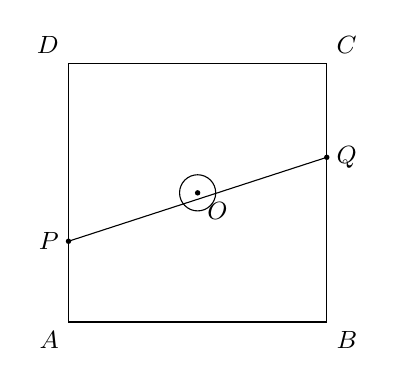
\begin{tikzpicture}[scale=0.82, every node/.style={font=\small}]
  \coordinate (A) at (0,0);
  \coordinate (B) at (4,0);
  \coordinate (C) at (4,4);
  \coordinate (D) at (0,4);
  \coordinate (O) at (2,2);
  \coordinate (P) at (0,1.25);
  \coordinate (Q) at (4,2.55);
  \draw (A)--(B)--(C)--(D)--cycle;
  \draw (O) circle[radius=0.28];
  \draw (P)--(Q);
  \fill (O) circle (1.2pt);
  \fill (P) circle (1.2pt);
  \fill (Q) circle (1.2pt);
  \node[below left] at (A) {$A$};
  \node[below right] at (B) {$B$};
  \node[above right] at (C) {$C$};
  \node[above left] at (D) {$D$};
  \node[below right] at (O) {$O$};
  \node[left] at (P) {$P$};
  \node[right] at (Q) {$Q$};
\end{tikzpicture}
\end{center}
\nopagebreak[4]
\end{question}
\gkpart{二、选择题}

（本大题共 4 题，每题 5 分，共 20 分。）

\begin{question}
\gkti{13}下列函数中，为偶函数的是\mbox{（　　）}。

（A）$y=x^{-2}$　　（B）$y=x^{1/3}$　　（C）$y=x^{-1/2}$　　（D）$y=x^3$

\Needspace{0.4\textheight}
\end{question}
\begin{question}
\gkti{14}如图，在直三棱柱 $ABC-A_1B_1C_1$ 的棱所在的直线中，与直线 $BC_1$ 异面的直线的条数为\mbox{（　　）}。

（A）1　　（B）2　　（C）3　　（D）4
\nopagebreak[4]
\begin{center}% Source: src-b19b233abb266d1b051ded3c332a399c1722d8192d07ce1bf2234dda57bd25bc, PDF p.2.
% Right triangular prism topology and the specified line BC_1; schematic projection.
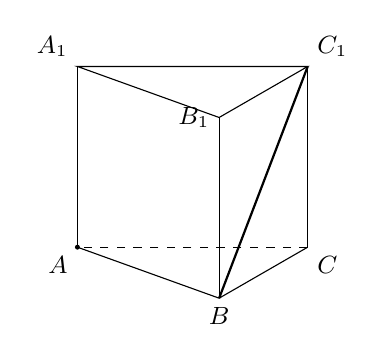
\begin{tikzpicture}[scale=0.9, every node/.style={font=\small}]
  \coordinate (A) at (0,0);
  \coordinate (B) at (2.0,-0.72);
  \coordinate (C) at (3.25,0);
  \coordinate (A1) at (0,2.55);
  \coordinate (B1) at (2.0,1.83);
  \coordinate (C1) at (3.25,2.55);
  \draw (A)--(B)--(C);
  \draw[dashed] (C)--(A);
  \draw (A1)--(B1)--(C1)--cycle;
  \draw (A)--(A1) (B)--(B1) (C)--(C1);
  \draw[thick] (B)--(C1);
  \fill (A) circle (1pt);
  \node[below left] at (A) {$A$};
  \node[below] at (B) {$B$};
  \node[below right] at (C) {$C$};
  \node[above left] at (A1) {$A_1$};
  \node[left] at (B1) {$B_1$};
  \node[above right] at (C1) {$C_1$};
\end{tikzpicture}
\end{center}
\nopagebreak[4]
\end{question}
\begin{question}
\gkti{15}设 $S_n$ 为数列 $\{a_n\}$ 的前 $n$ 项，“$\{a_n\}$ 是递增数列”是“$\{S_n\}$ 是递增数列”的\mbox{（　　）}。

（A）充分非必要条件　　（B）必要非充分条件

（C）充要条件　　（D）既非充分又非必要条件

\end{question}
\begin{question}
\gkti{16}已知 $A\text{、}B$ 为平面上的两个定点，且 $|\overrightarrow{AB}|=2$，该平面上的动线段 $PQ$ 的端点 $P\text{、}Q$，满足 $|\overrightarrow{AP}|\leq 5$，$\overrightarrow{AP}\cdot\overrightarrow{AB}=6$，$\overrightarrow{AQ}=-2\overrightarrow{AP}$，则动线段 $PQ$ 所形成图形的面积为\mbox{（　　）}。

（A）36　　（B）60　　（C）72　　（D）108

\end{question}
\gkpart{三、解答题}

（本大题共 5 题，共 $14+14+14+16+18=76$ 分。）

\begin{question}
\gkti{17}已知 $y=\cos x$。

（1） 若 $f(\alpha)=\dfrac13$，且 $\alpha\in[0,\pi]$，求 $f\left(\alpha-\dfrac\pi3\right)$ 的值；

（2） 求函数 $y=f(2x)-2f(x)$ 的最小值。

\begin{gktip}
原文未见 $f$ 的显式定义；此处保持“已知 $y=\cos x$”原文，不补为 $f(x)=\cos x$。
\end{gktip}

\end{question}
\begin{question}
\gkti{18}已知 $a\in\mathbb R$，双曲线 $\Gamma:\dfrac{x^2}{a^2}-y^2=1$。

（1） 若点 $(2,1)$ 在上，求 $\Gamma$ 的焦点坐标；

（2） 若 $a=1$，直线 $y=kx+1$ 与 $\Gamma$ 相交于 $A\text{、}B$ 两点，且线段 $AB$ 中点的横坐标为 1，求实数 $k$ 的值。

\begin{gktip}
原文“若点 $(2,1)$ 在上”未在“在上”之间标出曲线名称；此处照录，不补入 $\Gamma$。
\end{gktip}

\Needspace{0.4\textheight}
\end{question}
\begin{question}
\gkti{19}利用“平行于圆锥母线的平面截圆锥面，所得截线是抛物线”的几何原理，某快餐店用两个射灯（射出的光锥为圆锥）在广告牌上投影出某标识，如图1所示，图2是投影射出的抛物线的平面图，图3是一个射灯投影的直观图，在图2与图3中，点 $O\text{、}A\text{、}B$ 在抛物线上，$OC$ 是抛物线的对称轴，$OC\perp AB$ 于 $C$，$AB=3$ 米，$OC=4.5$ 米。

（1） 求抛物线的焦点到准线的距离；

（2） 在图3中，已知 $OC$ 平行于圆锥的母线 $SD$，$AB\text{、}DE$ 是圆锥底面的直径，求圆锥的母线与轴的夹角大小（精确到 $0.01^\circ$）。
\nopagebreak[4]
\begin{center}% Source: src-b19b233abb266d1b051ded3c332a399c1722d8192d07ce1bf2234dda57bd25bc, PDF p.4.
% Include the source-context photograph as a raster asset; mathematical diagrams are redrawn separately.
\begin{center}
  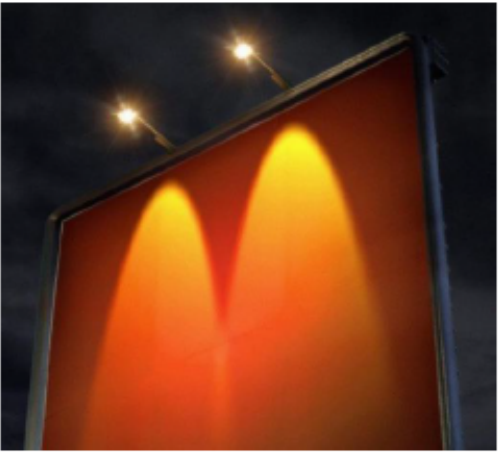
\includegraphics[width=0.46\linewidth]{assets/f2018_shanghai_spring_q19_photo.png}
\end{center}
\end{center}
\nopagebreak[4]
\nopagebreak[4]
\begin{center}% Source: src-b19b233abb266d1b051ded3c332a399c1722d8192d07ce1bf2234dda57bd25bc, PDF p.4.
% Reproduces the labeled parabola relation; curve shape and offset context are schematic.
\begin{tikzpicture}[scale=0.82, every node/.style={font=\small}]
  \coordinate (O) at (0,2.8);
  \coordinate (A) at (-1.2,0);
  \coordinate (B) at (1.2,0);
  \coordinate (C) at (0,0);
  \draw[densely dashed, domain=-2.55:-1.25, samples=60, variable=\x]
    plot (\x,{2.8-1.95*(\x+1.25)^2});
  \draw[thick, domain=-1.2:1.2, samples=80, variable=\x]
    plot (\x,{2.8-1.95*\x^2});
  \draw (A)--(B);
  \draw (O)--(C);
  \draw (0,0.18)--(0.18,0.18)--(0.18,0);
  \fill (O) circle (1pt);
  \fill (A) circle (1pt);
  \fill (B) circle (1pt);
  \node[above] at (O) {$O$};
  \node[below left] at (A) {$A$};
  \node[below right] at (B) {$B$};
  \node[below right] at (C) {$C$};
\end{tikzpicture}
\end{center}
\nopagebreak[4]
\nopagebreak[4]
\begin{center}% Source: src-b19b233abb266d1b051ded3c332a399c1722d8192d07ce1bf2234dda57bd25bc, PDF p.4.
% Cone topology and parallel OC/SD relation; projection is schematic, not metric.
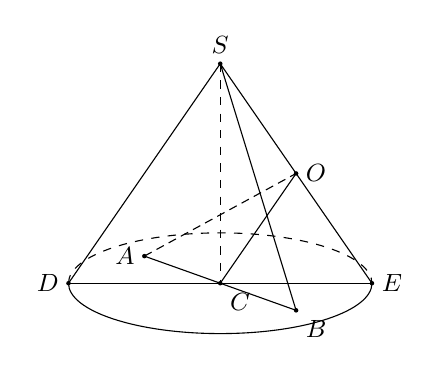
\begin{tikzpicture}[scale=0.82, every node/.style={font=\small}]
  \coordinate (S) at (0,3.4);
  \coordinate (D) at (-2.35,0);
  \coordinate (E) at (2.35,0);
  \coordinate (C) at (0,0);
  \coordinate (A) at (-1.175,0.42);
  \coordinate (B) at (1.175,-0.42);
  \coordinate (O) at (1.175,1.7);
  \draw (S)--(D) (S)--(E) (S)--(B);
  \draw[dashed] (S)--(C);
  \draw (D) arc[start angle=180,end angle=360,x radius=2.35,y radius=0.78];
  \draw[dashed] (D) arc[start angle=180,end angle=0,x radius=2.35,y radius=0.78];
  \draw (D)--(E);
  \draw (A)--(B);
  \draw (C)--(O);
  \draw[densely dashed] (A)--(O);
  \fill (S) circle (1pt);
  \fill (D) circle (1pt);
  \fill (E) circle (1pt);
  \fill (A) circle (1pt);
  \fill (B) circle (1pt);
  \fill (C) circle (1pt);
  \fill (O) circle (1pt);
  \node[above] at (S) {$S$};
  \node[left] at (D) {$D$};
  \node[right] at (E) {$E$};
  \node[left] at (A) {$A$};
  \node[below right] at (B) {$B$};
  \node[below right] at (C) {$C$};
  \node[right] at (O) {$O$};
\end{tikzpicture}
\end{center}
\nopagebreak[4]
\end{question}
\begin{question}
\gkti{20}设 $a>0$，函数 $f(x)=\dfrac{1}{1+a\cdot2^x}$。

（1） 若 $a=1$，求 $f(x)$ 的反函数 $f^{-1}(x)$；

（2） 求函数 $y=f(x)\cdot f(-x)$ 的最大值（用 $a$ 表示）；

（3） 设 $g(x)=f(x)-f(x-1)$，若对任意 $x\in(-\infty,0]$，$g(x)\geq g(0)$ 恒成立，求 $a$ 取值范围。

\end{question}
\begin{question}
\gkti{21}若 $\{c_n\}$ 是递增数列，数列 $\{a_n\}$ 满足：对任意 $n\in\mathbb N^*$，存在 $m\in\mathbb N^*$，使得
\nopagebreak[4]
\[
\frac{a_m-c_n}{a_m-c_{n+1}}\leq0,
\]
则称 $\{a_n\}$ 是 $\{c_n\}$ 的“分隔数列”。

（1） 设 $c_n=2n$，$a_n=n+1$，证明：数列 $\{a_n\}$ 是 $\{c_n\}$ 的分隔数列；

（2） 设 $c_n=n-4$，$S_n$ 是 $\{c_n\}$ 的前 $n$ 项和，$d_n=c_{3n-2}$，判断数列 $\{S_n\}$ 是否是数列 $\{d_n\}$ 的分隔数列，并说明理由；

（3） 设 $c_n=aq^{n-1}$，$T_n$ 是 $\{c_n\}$ 的前 $n$ 项和，若数列 $\{T_n\}$ 是 $\{c_n\}$ 的分隔数列，求实数 $a\text{、}q$ 的取值范围。

\begin{gktip}
原卷第 6 页明确印有“前 $n$ 项和”；此前转录漏掉“和”字，现已按原页更正。
\end{gktip}

\end{question}